\subsection{Page conditioning and line segmentation}
\label{sec:des-seg}
The recogniser requires an image containing one line of text. A photograph, however, may contain uneven illumination, a rotated page, printed rules, page edges and strokes extending between neighbouring lines. The purpose of this stage is to remove those disturbances while preserving the shape and relative spacing of the handwriting. The implemented sequence in \texttt{segment.py} works mainly on a half-resolution image, then returns to the full-resolution image to build the line crops.

\subsubsection{Input conditions and processing sequence}
The working image is a two-dimensional array of grey values. Where a colour array reaches the deskew routine, its channels are averaged to obtain brightness. Reducing the analysis image by averaging each $2\times2$ block reduces its pixel count by a factor of four. Averaging is preferred to selecting every second pixel because a thin stroke then contributes to the reduced image even if it falls between sampling positions. A further reduced mask is sufficient for the angle search, where only the arrangement of whole lines is needed.

The intermediate representations in Figure~\ref{fig:des-seg-stages} separate illumination correction, ink extraction, line boundaries and final crops. Inspecting these representations localises a missing stroke to the operation that removed it. The output includes the line images together with their order and diagnostic information such as skew angle, pitch and rejected crops.

\begin{figure}[!htbp]\centering
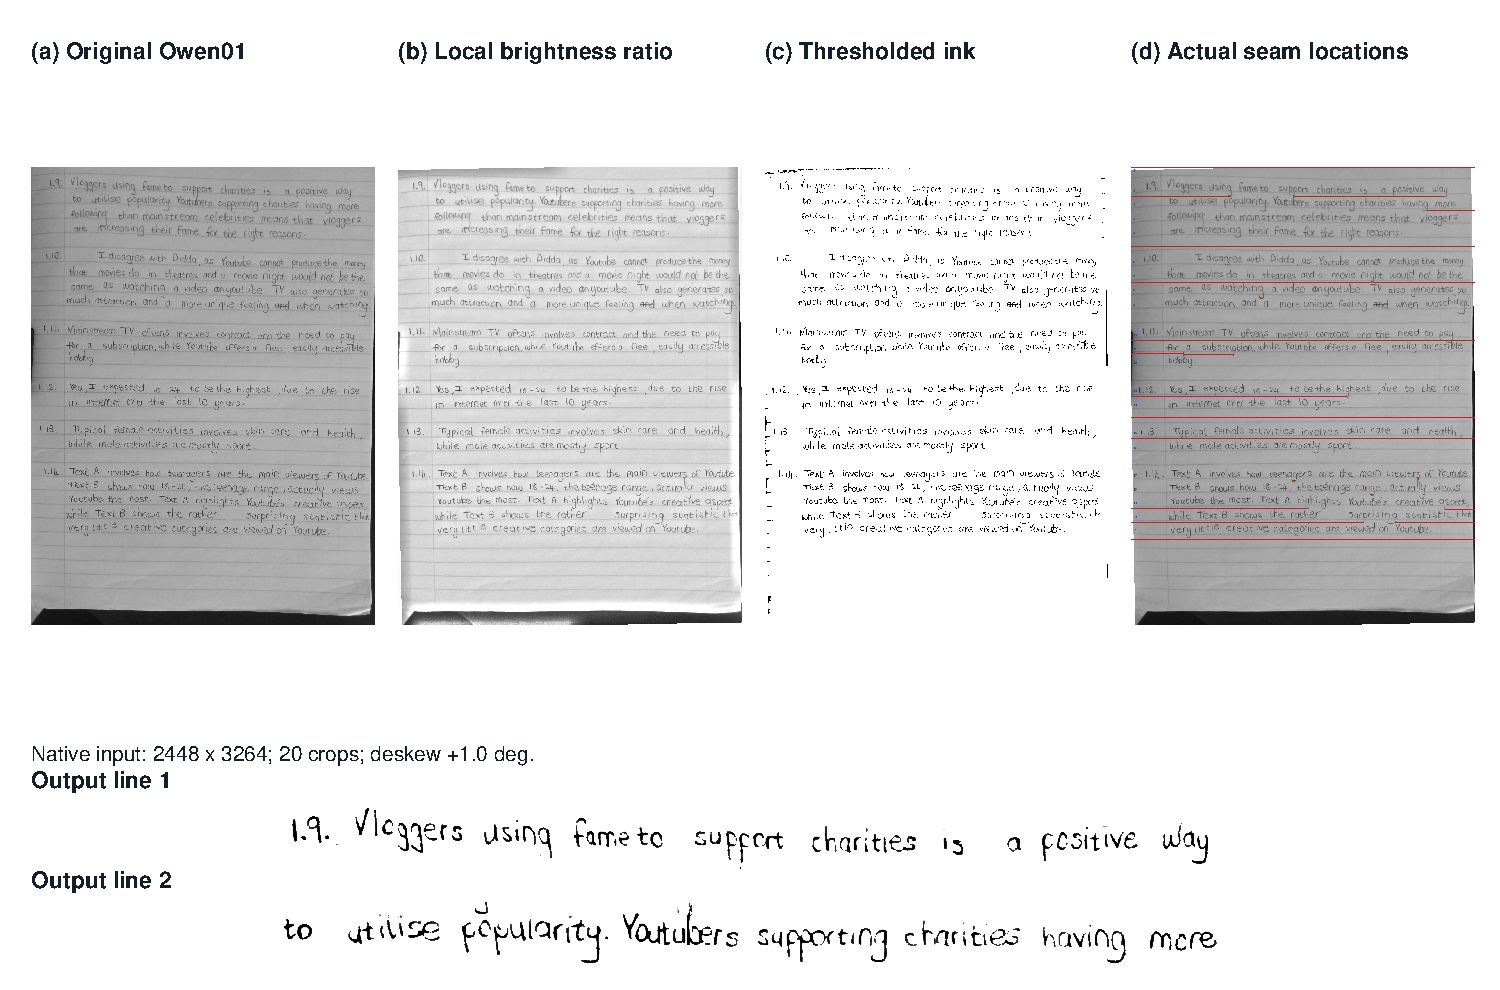
\includegraphics[width=0.96\linewidth]{Figures/design-segmentation-stages.pdf}
\caption{Processing stages used to obtain separate text-line images from a photographed page.}
\label{fig:des-seg-stages}
\end{figure}

A straight horizontal boundary is adequate only when there is a blank row between lines. Handwritten descenders and ascenders can overlap in vertical position without belonging to the same line. The chosen design first locates the lines, finds curved boundaries between them, then uses component geometry to refine which line owns each ink piece. This is more appropriate than treating every connected ink component as a character, since cursive words may form a single component.

Algorithm~\ref{alg:des-segment} links the representations used in Figure~\ref{fig:des-seg-stages}. The order matters: rules and artefacts are removed before estimating final line centres, whereas faint-ink recovery occurs after ownership has been established.

\begin{designalgorithm}
\caption{Photographed page to ordered line crops}
\label{alg:des-segment}
\prequire{Grey page on its chosen line axis.}
\pensure{Ordered full-resolution crops, coordinates and diagnostics.}
\begin{designpseudo}
\pstate{0}{$(G_f,G_h,M,R,\theta)\leftarrow\operatorname{Deskew}(G)$}
\pstate{0}{$M\leftarrow\operatorname{RemovePrintedStructure}(M,G_h)$}
\pstate{0}{$(M,\mathcal C)\leftarrow\operatorname{DropArtifactPieces}(M,R)$}
\pstate{0}{$(P,c)\leftarrow\operatorname{LineCentres}(M)$}
\pstate{0}{$b\leftarrow\operatorname{SeamCuts}(M,c,P)$}
\pstate{0}{$O\leftarrow\operatorname{AssignOwnership}(M,\mathcal C,b,c,P)$}
\pstate{0}{$\mathcal L\leftarrow\varnothing$; normalise full-resolution brightness}
\pstate{0}{\textbf{for each} line index $n$ \textbf{do}}
\pstate{1}{$C_n\leftarrow\operatorname{BuildLineCrop}(n,O,G_f,P)$}
\pstate{1}{\textbf{if} $C_n$ has sufficient ink and height \textbf{then}}
\pstate{2}{Append $C_n$, its fixed-canvas view and bounding box to $\mathcal L$}
\pstate{1}{\textbf{end if}}
\pstate{0}{\textbf{end for}}
\pstate{0}{$\mathcal L\leftarrow\operatorname{DropSolidCrops}(\mathcal L)$; renumber retained crops}
\pstate{0}{\textbf{return} $\mathcal L$, seams, ratio image and diagnostics}
\end{designpseudo}
\end{designalgorithm}

\subsubsection{Lighting normalisation and ink extraction}
The first requirement is to distinguish ink from paper under an illumination gradient. A single threshold applied directly to brightness can classify a shadowed part of the page as ink while losing pale strokes elsewhere. Local-mean comparison addresses this illumination problem in adaptive thresholding~\cite[pp.~2--3]{bradley2007}. The present design instead forms a local brightness ratio and selects its threshold from the ratio histogram. Equation~\ref{eq:des-ratio} compares each pixel with its own local background estimate instead.
\begin{equation}
R(y,x)=\frac{G(y,x)}{\max[B_r(y,x),1]},\qquad
M(y,x)=\mathbf{1}[R(y,x)<t^*].
\label{eq:des-ratio}
\end{equation}
In the Owen01 page trace, pixel $(y,x)=(317,343)$ of the $800\times600$ pre-deskew working image has $G=100$. Its 41 by 41 background window gives $B_r=161.43367$, hence $R=100/161.43367=0.619449$. The selected ratio threshold is $0.803906$, so this pixel enters the ink mask. The trace uses the documented reduction of the stored photograph.

Here $G$ is grey intensity on the 0--255 scale, $B_r$ is a square-window mean with radius $r$, $R$ is normalised brightness, and $M$ is the binary ink mask. The floor of 1 prevents division by zero in black regions. The code uses $r=\max(8,\min(40,\operatorname{round}(H/41)))$, where $H$ is the working-image height. The radius follows image size within bounded limits: it must average over strokes without following their darkness as if it were illumination.

The mean is evaluated through a summed-area table, using the four-corner rectangle sum described by Bradley and Roth~\cite[p.~2]{bradley2007}. For an exclusive prefix sum $S$, the window sum is obtained from four accesses, as shown in Equation~\ref{eq:des-integral}.
\begin{equation}
\Sigma_{[y_0,y_1)\times[x_0,x_1)}=
S(y_1,x_1)-S(y_0,x_1)-S(y_1,x_0)+S(y_0,x_0).
\label{eq:des-integral}
\end{equation}
The same pixel's four prefix values are $20696850$, $18404173$, $18359673$ and $16338366$. Equation~\ref{eq:des-integral} gives a window sum of $271370$, so $B_r=271370/1681=161.43367$. This is the local-background value used in the preceding mask decision.

The window area divides this sum to give $B_r$. Equation~\ref{eq:des-integral} makes the cost per window independent of its radius after the prefix image has been constructed. Edge replication is used by this local-mean routine so that the boundary is not darkened by artificial zero padding.

Otsu's criterion selects $t^*$ from the ratio histogram rather than from the original grey histogram~\cite{otsu1979}. Equation~\ref{eq:des-otsu} gives the between-class variance being maximised.
\begin{equation}
t^*=\arg\max_t\ \omega_0(t)\omega_1(t)
\bigl[\mu_0(t)-\mu_1(t)\bigr]^2.
\label{eq:des-otsu}
\end{equation}
For this page's ratio histogram, the selected bin is 171. Its masses are $\omega_0=0.07069375$ and $\omega_1=0.92930625$, with mean bin indices 124.98356 and 217.71913. Their between-class variance is approximately $564.97942$ in squared bin-index units. Converting the selected bin centre to the ratio scale gives $t^*=(171+0.5)(1.2/256)=0.80390625$, the threshold used above.

Here $\omega_0,\omega_1$ are the histogram masses below and above a candidate threshold and $\mu_0,\mu_1$ are their means. The normalisation in Equation~\ref{eq:des-ratio} first brings paper towards a common level, allowing the global criterion in Equation~\ref{eq:des-otsu} to operate on a more consistent image. The implementation uses 256 bins over the clipped ratio range 0--1.2.

Large solid regions are then removed because the dark surround or a binder interior can survive thresholding without representing handwriting. The page region is estimated from its bright connected area, and long nearly horizontal or vertical ink runs are masked as printed structure. Run thresholds are expressed relative to line pitch, rather than fixed photograph dimensions. The horizontal and vertical limits are respectively 1.25 and 1.4 pitches. These are geometric heuristics: a long handwritten underline can satisfy the same condition as a printed rule, so the algorithm is designed for text extraction rather than preserving every mark on a page.

\subsubsection{Page orientation and skew correction}
Orientation is treated at two scales. A quarter turn changes which axis contains the line gaps; a small skew changes how sharply ink is concentrated along rows. For the quarter-turn decision, the code compares the fraction of nearly empty rows in the current image and its $90^\circ$ rotation. A turn is accepted only when the rotated score exceeds the original by a factor of 1.35. This margin avoids rotating a page merely because two weak scores differ slightly. Sparse or unusually arranged text can still make the row-gap evidence ambiguous.

After choosing the line axis, the deskew routine tests angles from $-4^\circ$ to $+4^\circ$ at $0.5^\circ$ spacing. Equation~\ref{eq:des-skew} gives its objective, related to projection-profile methods~\cite{postl1986}.
\begin{equation}
\theta^*=\arg\max_\theta\sum_y p_\theta(y)^2,\qquad
p_\theta(y)=\sum_x M_\theta(y,x).
\label{eq:des-skew}
\end{equation}
The Owen01 angle search gave squared-projection scores of 442973 at $+0.5^\circ$, 464105 at $+1.0^\circ$ and 439403 at $+1.5^\circ$. The maximum over all seventeen tested angles was 464105, so the routine selected $+1.0^\circ$. These scores are computed from the reduced mask used by the angle search, before the final mask is rebuilt.

Here $p_\theta$ is the row ink count at a candidate angle. Squaring favours concentrated rows over the same amount of ink spread across many rows. Rather than rotating the complete mask for every trial, the implementation maps ink coordinates to candidate rows and counts them. The selected rotation is then applied to the full and working grey images, and the mask is recomputed. This avoids repeatedly interpolating a binary image.

A page and its upside-down version have the same line-axis structure. The server therefore uses the reader to compare up to three sampled line crops in both directions. It compares the mean best-frame log score, reuses the selected readings and reverses line order when necessary. This is an orientation heuristic, not an independent measure of text correctness. A reader that is confidently wrong can select the wrong orientation, particularly when little text is available.

\subsubsection{Line detection and separation}
The line pitch $P$ provides the main scale reference for later decisions. A smoothed row profile is formed from the central writing region; candidate peaks must exceed 6\% of its maximum. The preferred estimate is the median distance between peaks, subject to a lower bound based on component height. This check prevents the ascender, body and descender bands of a single large line from being treated as separate line spacings. Autocorrelation and a component-height estimate provide fallbacks when direct gaps are unsuitable.

Line centres are selected in order of peak strength, with a minimum separation of $0.6P$. This suppresses several peaks within the same line. The code also supports merging peaks separated by a shallow valley, but that additional rule is not automatically active for every photographed page; its default threshold disables merging. The distinction matters because a rule that improves rendered text need not improve the shadows and artefacts of a real photograph.

Between each pair of centres, a minimum-cost seam crosses the image from left to right. The dynamic programme in Equation~\ref{eq:des-seam} follows the seam-carving principle~\cite[p.~3]{avidan2007}.
\begin{equation}
D(y,x)=C(y,x)+\min_{|d|\leq s}
\{D(y+d,x-1)+0.02|d|\}.
\label{eq:des-seam}
\end{equation}
In the traced boundary between centres 38 and 61, the selected predecessor at column 283 changes from row 50 to row 49 in working-image coordinates. Its stored predecessor cost is $0.00641966$, the movement penalty is $0.02$ and the new local cost is $0.0000226843$. Equation~\ref{eq:des-seam} therefore gives $D\simeq0.00641966+0.02+0.0000226843=0.02644234$. This traces one selected minimum of the actual dynamic programme; equal-cost alternatives can also occur.

Here $D$ is accumulated cost, $C$ is the local cost and $s=7$ is the allowed row change per column. Backtracking from the minimum final cost returns the boundary. Equation~\ref{eq:des-seam} penalises unnecessary vertical movement while allowing a boundary to bend around a descender.

The project-specific cost in Equation~\ref{eq:des-seamcost} combines an ink-crossing penalty with a weaker attraction to the space between line centres. These terms adapt the minimum-cost seam principle to the detected text-line gaps; the weights are engineering choices examined by the sensitivity check below.
\begin{equation}
C(y,x)=4\widetilde M(y,x)
+0.012\left(\frac{y-y_m}{h_g}\right)^2.
\label{eq:des-seamcost}
\end{equation}
At that boundary point, $y_m=(38+61)/2=49.5$, $h_g=(61-38)/2=11.5$ and the closed mask is zero. The implemented local cost is therefore $C=0.012[(49-49.5)/11.5]^2=0.0000226843$. It provides the local term used in the preceding accumulated-cost calculation.

Here $\widetilde M$ is the mask after morphological closing, a dilation followed by erosion that fills narrow breaks and gaps~\cite[p.~541]{haralick1987}, $y_m$ is the midpoint of the neighbouring centres and $h_g$ is half their separation. The closing radius is $\max(2,\lfloor0.07P\rfloor)$ pixels. Closing fills narrow gaps that would otherwise let a seam enter a stroke, without simply treating a thick dilation around every letter as real ink. In Equation~\ref{eq:des-seamcost}, the midpoint term resolves low-ink alternatives; it is deliberately much weaker than the ink penalty. The examples in Section~\ref{sec:des-segverify} examine the resulting boundaries and the cases that still defeat these geometric preferences.

A new sensitivity check on six fixed gaps from two real pages varies the midpoint and step penalties separately. At the implemented 0.012/0.02 setting, mean midpoint offset is 0.363 working pixels; removing the midpoint attraction raises it to 4.055 pixels. All tested settings still cross two raw-ink pixels across those seams, so this checks the weights' effects rather than proving an optimum. Appendix~\ref{app:des-seam-sweep} gives the settings and retained outcomes.

Figure~\ref{fig:vt-seamfield} shows why the curved boundary is useful on Abhinav01 at native page resolution. Among that page's gaps, the first example was selected for the largest reduction in crossed ink: the midpoint cut intersects 64 working-image ink pixels, while the seam intersects one. The second was selected for the largest departure from the midpoint; its seam moves by up to 22 rows and crosses no ink, compared with 44 pixels for the straight cut. These selected examples expose the effect of the cost function rather than establishing an average segmentation improvement.

\begin{figure}[!htbp]\centering
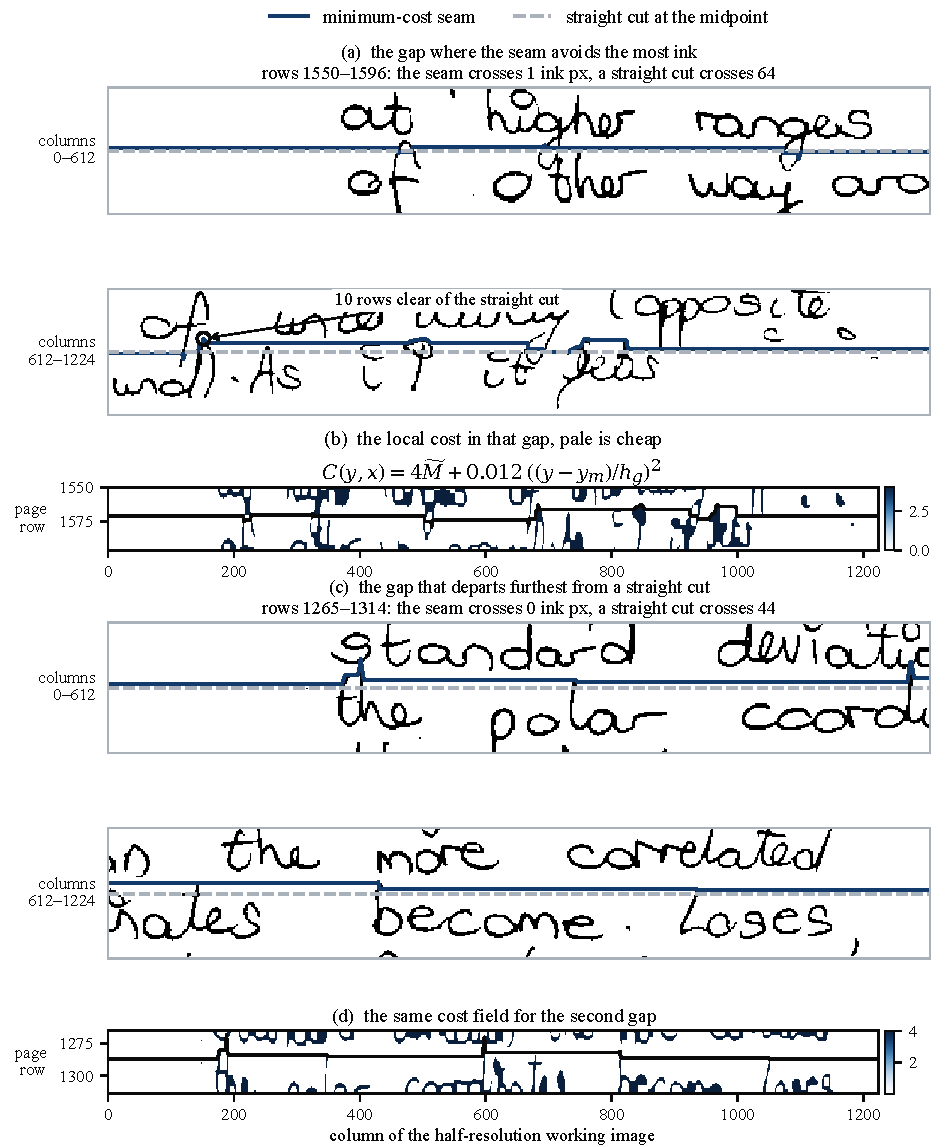
\includegraphics[width=\linewidth]{Figures/VisualTests/T25_seam_cost_field.pdf}
\caption{Seam paths and local cost fields on two explicitly selected gaps from Abhinav01.}
\label{fig:vt-seamfield}
\end{figure}

\subsubsection{Ink ownership and classifier crop preparation}
Seams initially divide the image into bands, but a pixel-by-pixel cut can separate a dot from its stem or clip a curved descender. Connected-component ownership therefore refines the band assignment. Components are found with row runs and union operations, following connected-component labelling principles~\cite[pp.~476--479]{rosenfeld1966}. The implementation includes diagonal contact, giving eight-connected components. Large pieces can still contain writing from more than one line, so component labelling alone is not a complete line assignment.

Algorithm~\ref{alg:des-ownership} summarises the correction order. For a component spanning several bands, a band holding at least 15\% of its in-band ink is substantial. The uppermost substantial band supplies the reference owner for small-piece corrections; otherwise the largest overlap is used. Large components are not indiscriminately moved into that band: their pixels retain seam-band assignment except where the small-piece and narrow-tail rules apply. This distinction preserves a word's main body while recovering a protruding part.

\begin{designalgorithm}
\caption{Refining seam bands into ink ownership}
\label{alg:des-ownership}
\prequire{Ink mask $M$, components $\mathcal C$, seams, centres and pitch $P$.}
\begin{designpseudo}
\pstate{0}{\textbf{for each} component $C\in\mathcal C$ \textbf{do}}
\pstate{1}{Count overlap $a_{C,n}$ with each seam band $n$}
\pstate{1}{$S\leftarrow\{n:a_{C,n}\geq0.15\sum_j a_{C,j}\}$}
\pstate{1}{Choose topmost $S$ as reference owner, or maximum overlap if $S=\varnothing$}
\pstate{1}{Correct eligible narrow tails and small pieces; reject remote specks}
\pstate{1}{Associate compact dots with plausible stems using pitch-scaled guards}
\pstate{0}{\textbf{end for}}
\pstate{0}{$O\leftarrow$ corrected ownership, preserving large-piece seam assignments}
\pstate{0}{\textbf{for each} raw component near a neighbouring line \textbf{do}}
\pstate{1}{\textbf{if} detached-dot or enclosed-ring guards pass \textbf{then}}
\pstate{2}{Transfer eligible pixels to the supported stem's line; protect correction}
\pstate{1}{\textbf{end if}}
\pstate{0}{\textbf{end for}}
\pstate{0}{Reassign residual fragments lacking their own body-band support}
\pstate{0}{\textbf{return} $O$; excluded pixels retain no line index}
\end{designpseudo}
\end{designalgorithm}

An \texttt{i} dot between two text lines illustrates the need for this sequence. A seam may put it with the upper line because of its vertical position, while a stem below supplies evidence for the lower line. Closing used for component analysis can also join the dot to an unrelated descender; the raw mask is therefore revisited rather than treating the closed component as unquestionable evidence. A ring-shaped mark needs the additional hole test so that an open hook is not treated as a detached loop. These are geometric decisions with ambiguous cases, rather than knowledge of the intended character.

The final crop is built from the full-resolution image and the refined ownership map. Contrast adjustment improves faint ink, while ownership restricts recovery so that strengthening one line does not simply pull a neighbouring stroke into it. The recogniser receives an aspect-preserving fit on a 64 by 640 canvas. Equation~\ref{eq:des-fit} defines the common scale for an original crop of height $h$ and width $w$.
\begin{equation}
a=\min\left(\frac{64}{h},\frac{640}{w}\right),\qquad
(h',w')\simeq(ah,aw).
\label{eq:des-fit}
\end{equation}
The archived first Owen01 line is $156\times2170$ pixels. Its fit scale is $a=\min(64/156,640/2170)=0.2949309$, giving a $46\times640$ resized image after integer rounding. The routine places it nine rows below the top of the 64-row canvas, retaining its aspect ratio and filling the remaining rows with white.

Remaining space is padded white, with the ink left-aligned and vertically centred. The shared scale in Equation~\ref{eq:des-fit} avoids stretching narrow letters differently from wide ones. Very long lines, however, become short in height when fitted to the width limit, which reduces the detail available to the networks.

The full-resolution crop uses a soft interpolation of its own ink mask to avoid jagged cut edges. A separate ownership exclusion is resized with nearest-neighbour interpolation: interpolating a yes/no ownership decision could partly return a neighbour's ink. Local thresholding can recover faint strokes within a neighbourhood of this line, but cannot recover ink already assigned to another line. Contrast is stretched between a robust ink level and paper level, followed by a darkness exponent of 0.55. This strengthens faint writing without replacing its geometry with a solid rectangular band.

The final solid-crop guard rejects a crop only when its dark-pixel fraction exceeds both 15\% and three times the page's median crop fraction. Requiring both prevents one unusually dense but genuine line from being rejected merely because other lines are sparse. This reduces the chance of a solid shadow receiving a strong writer vote in Section~\ref{sec:des-integration}. If every crop would be rejected, the implementation retains the input crop list; crop rejection is therefore a guard rather than a guarantee of valid text.

The three largest ownership corrections on Abhinav01 are displayed in Figure~\ref{fig:vt-ownership}. Colour identifies the assigned line, and the boxes locate pixels whose ownership changes after the component rules. Across the page, 462 pixels change assignment; the three boxed components contain 115, 78 and 73 pixels. The examples make the detached-piece and protruding-stroke corrections inspectable. No manually labelled pixel-ownership reference was supplied, so the reassignment count measures the action of the rules rather than their accuracy.

\begin{figure}[!htbp]\centering
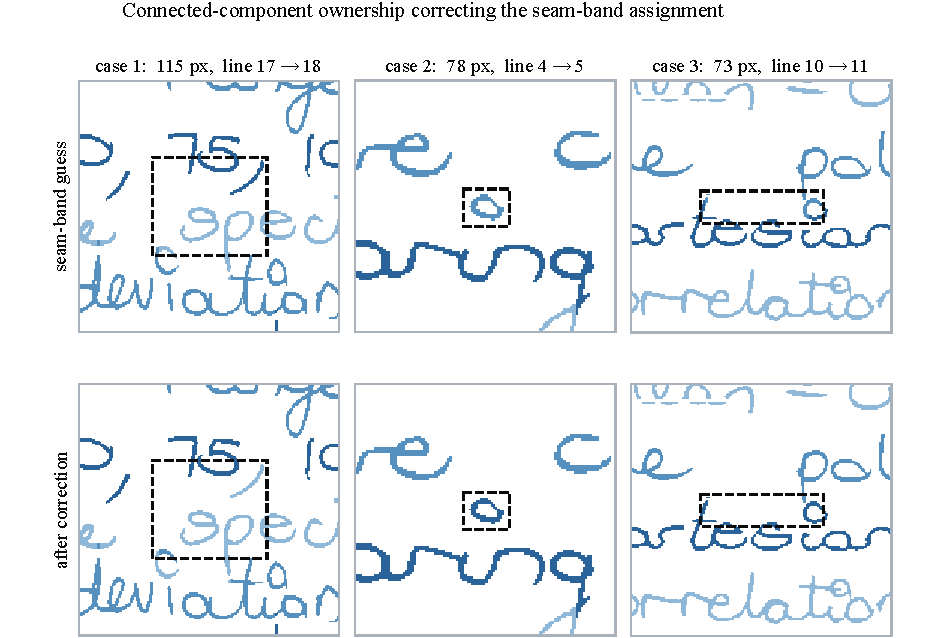
\includegraphics[width=\linewidth]{Figures/VisualTests/T27_ownership_corrections.pdf}
\caption{Initial seam-band ownership and corrected component ownership on the same page.}
\label{fig:vt-ownership}
\end{figure}

\subsubsection{Segmentation verification and limitations}
\label{sec:des-segverify}
Figure~\ref{fig:des-seg-variation} uses three actual photographs of the same three-line handwritten page from the camera roll. Their shadows and page presentation differ; no illuminance or physical rotation angle was recorded. The unchanged native images were processed through the line-axis decision and segmentation, without manually correcting an unsuccessful orientation.

The striped-shadow capture produced three crops. The diffuse-shadow capture produced four, so matching the writing visually remains necessary even under milder-looking illumination. The third capture was left on the wrong line axis: its gap scores were 0.379 and 0.400, giving a ratio of only 1.054 against the required 1.35, and segmentation produced 28 slices. Reaching the $-4^\circ$ deskew limit could not correct a missed quarter turn. These cases expose a sparse-page limitation of row-gap orientation; they do not establish a lighting operating range or a success rate. An acquisition guide or a separately verified orientation method would address the ambiguity before fine deskewing.

The fuller Owen page in Figure~\ref{fig:des-seg-stages} produced 20 crops at native resolution, matching its 20 labelled text lines. That count checks gross splitting, not every boundary pixel. Appendix~\ref{app:des-visual-tests} records the capture filenames, extended digital perturbations and independent algorithm checks, including failures after additional image reduction.

\begin{figure}[!htbp]\centering
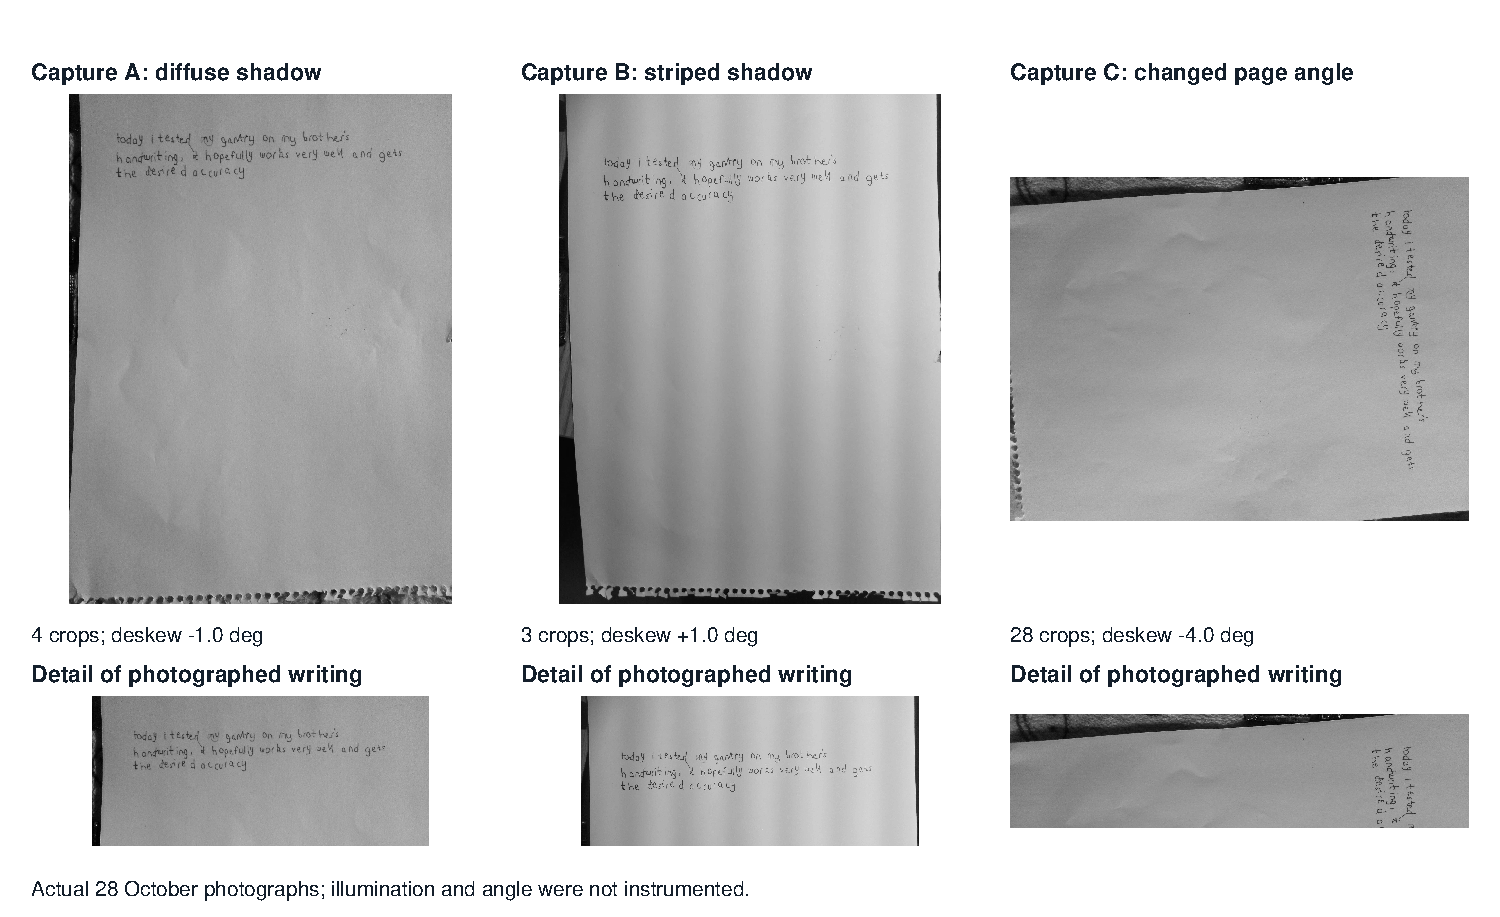
\includegraphics[width=0.95\linewidth]{Figures/design-segmentation-variation.pdf}
\caption{Actual repeated photographs and segmentation diagnostics for the same sparse page. Capture C retains the unsuccessful axis decision.}
\label{fig:des-seg-variation}
\end{figure}

The scale-based thresholds and curved boundaries accommodate changes in handwriting size and overlapping vertical extents without assigning every page a fixed pixel spacing. Their assumptions also define the limitations. Highly irregular line spacing weakens a single pitch estimate, touching strokes from two lines can defeat component ownership, and sparse pages provide weak orientation evidence. Severe perspective or page curvature is not corrected by a global rotation. Improving the mount addresses the latter at source; more general page rectification would add processing and require its own verification.
\FloatBarrier
